\noindent

 \section{Prediction framework}
 \label{prediction_1}
 


  
 \begin{figure*}
 \centering
   \includegraphics*[width=0.75\textwidth,angle=0]{./texfiles/Chapter_1/fig/age_all_5-eps-converted-to.pdf}
%    \hspace{20mm}(A)\hspace{20mm}(B)\hspace{20mm}(C)\hspace{20mm}(D)\hspace{20mm}(E)
 \caption{\label{aging}The average neighborhood-overlap value at different lags for (A)INFOCOM 2006, (B)SIGCOMM 2009, (C)Highschool 2012, (D)Highschool 2011 and (E)Hospital datasets.}
%\end{center}
 \end{figure*}

%  \begin{figure}
%  \begin{center}
%   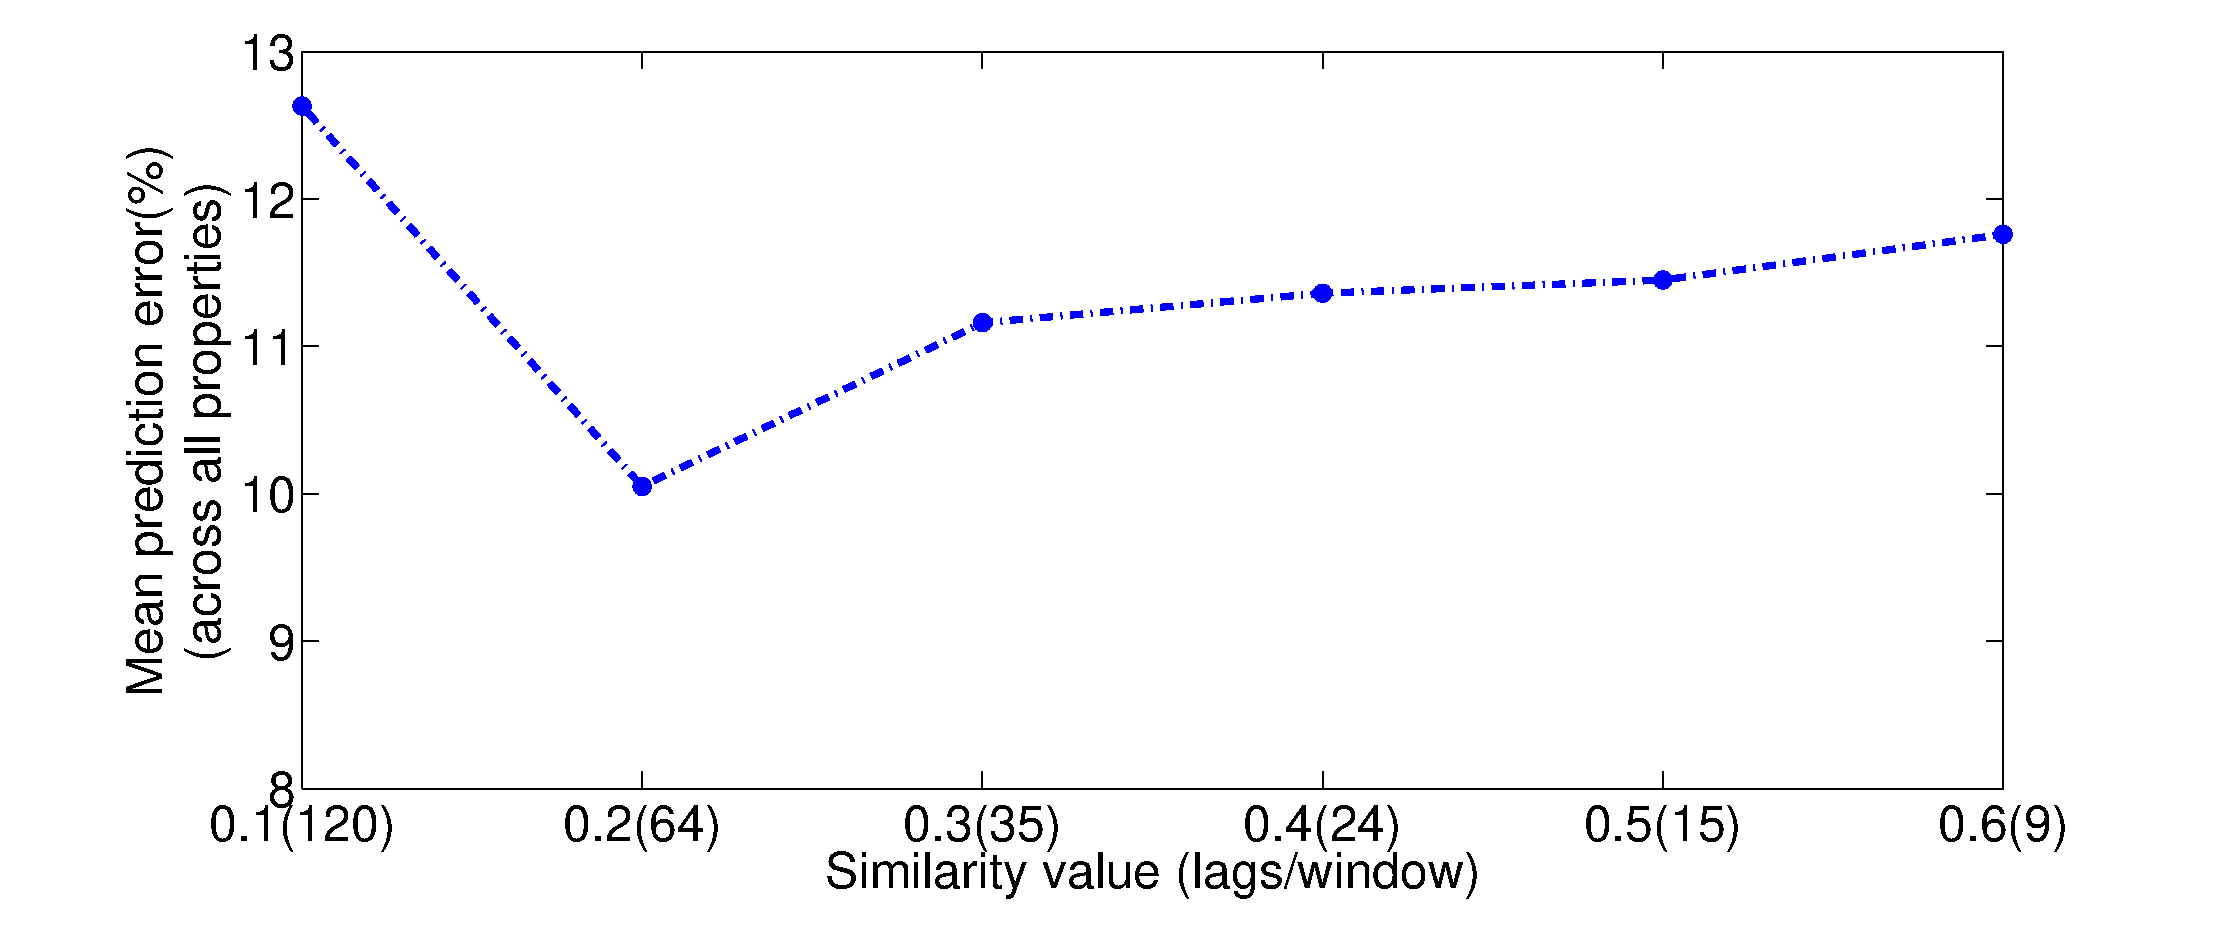
\includegraphics[width=0.75\columnwidth, angle=0]{fig/error_similarity_val.eps}
%   \caption{\label{fig_err} Mean prediction error (\%) across different properties for INFOCOM 2006 dataset for different similarity values. The lags corresponding to the similarity 
%   value are also provided.}
%   \end{center}
%  \end{figure}




% \begin{figure*}
%   \centering
%   \includegraphics*[width=0.95\textwidth,angle=0]{fig/error_dist_all.eps}
%  
%  %\hspace{8mm}(a)\hspace{60mm}(b)
%  
%  \caption{\label{fig8}  The percentage error distribution of all the properties (time series) for (A) INFOCOM 2006 dataset, (B) SIGCOMM 2009 dataset, (C) High-school 2011. (D) High-school 2012 and (E) Hospital. 
%  X-axis represents percentage error and Y-axis represents 
%  probability.}
% \end{figure*} 
  
In this section, we employ the time series to forecast the different structural properties of the temporal networks.
%Note that this process is equivalent to having a growth model for the temporal networks.
Elementary models of time series forecasting could be categorized into Auto-regressive (AR) and Moving average (MA) models ~\cite{chatfield2013analysis}. In case of 
an auto-regressive model of order $p$, AR($p$), the value of the time series at time step $t$ is given as - 
\begin{center}
 $y_{t}=\alpha_{1}y_{t-1}+\cdots+\alpha_{p}y_{t-p}+e_t+c$
\end{center}
where $\alpha_{i}$s are parameters, $e_t$ is the white noise error term and $c$ is a constant.
Similarly, in case of moving average model of order $q$, MA($q$), the value of the time series at time step $t$ is given as - 
\begin{center}
 $y_{t}=\beta_{1}e_{t-1}+\cdots+\beta_{q}e_{t-q}+\mu+e_t+c$
\end{center}
where $\beta_{i}$s are parameters, $e_t,e_{t-1},...$ are white noise error terms and $\mu$ is the expectation of $y_t$.
These two models could be combined into Auto-regressive-moving-average (ARMA($p$,$q$)) ~\cite{chatfield2013analysis} where the value of the time series at time step $t$ is given as
\begin{center}
 $y_{t}=\alpha_{1}y_{t-1}+\cdots+\alpha_{p}y_{t-p}+\beta_{1}e_{t-1}+\cdots+\beta_{q}e_{t-q}+e_t+c$
\end{center}

However, in our case the time series show evidences of non-stationarity and short term dependencies and these models are insufficient and hence we use ARIMA model ~\cite{box2011time} for forecasting. The initial differencing step in ARIMA model 
is used to reduce the non-stationarity.
%Any ARIMA model has three parameters $p$, $d$ and $q$. $p$ is the auto-regressive element representing the lingering effects of preceding scores.
%$d$ represents the integrated element and $q$ represents the moving average element.
On fitting an ARIMA($p$,$d$,$q$) model to a time series we obtain an auto-regressive 
equation of the form-

\begin{center}
 $y_{t}=\alpha_{1}y_{t-1}+\cdots+\alpha_{p}y_{t-p}+\beta_{1}e_{t-1}+\cdots+\beta_{q}e_{t-q}+c$
\end{center}

 \begin{figure}
 \begin{center}
  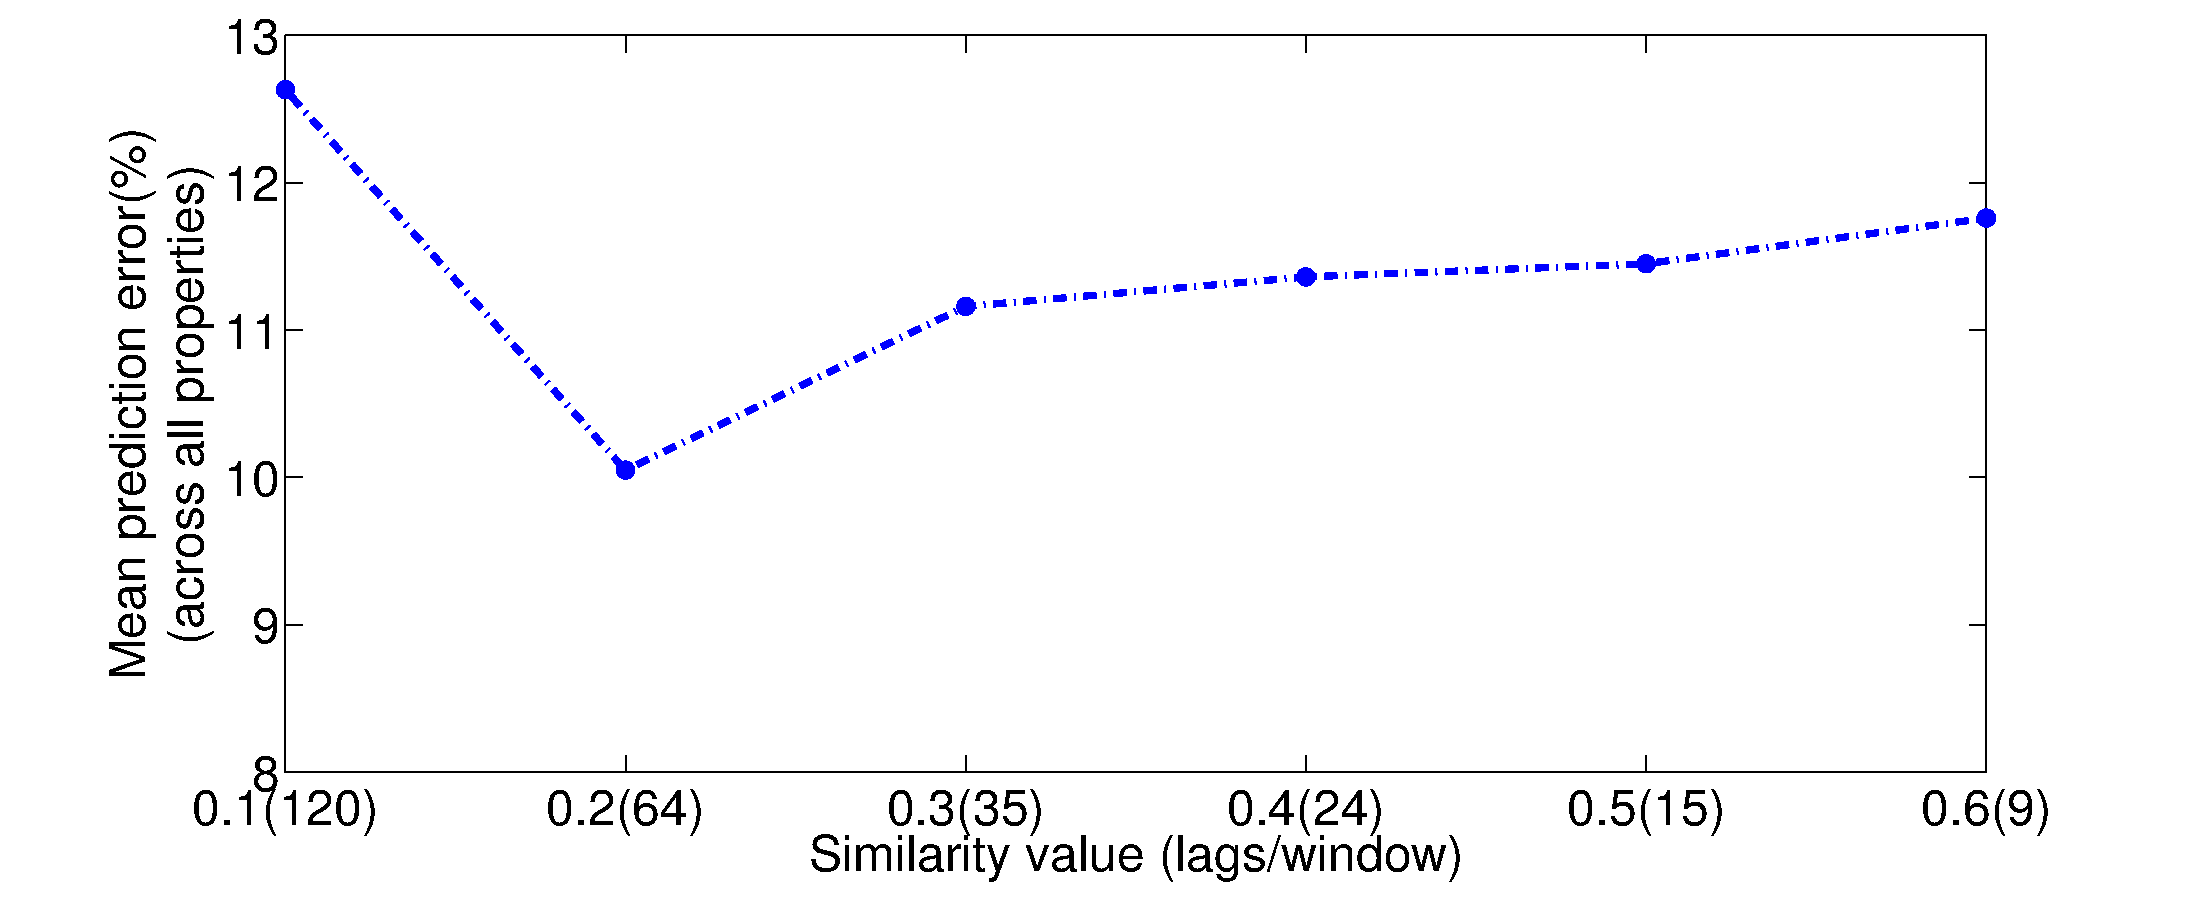
\includegraphics[width=0.75\columnwidth, angle=0]{./texfiles/Chapter_1/fig/error_similarity_val-eps-converted-to.pdf}
  \caption{\label{fig_err} Mean prediction error (\%) across different properties for INFOCOM 2006 dataset for different similarity values. The lags corresponding to the similarity 
  value are also provided.}
  \end{center}
 \end{figure}
 
Hence we can take a time series corresponding to a network property and fit an ARIMA model to it. Thus, we obtain an auto-regressive equation for that series which 
can be used 
in forecasting. 
% Note that our forecast results are performed on INFOCOM 2006 and SIGCOMM 2009 datasets. 
% For the Twitter hashtag co-occurrence dataset we find the time series corresponding to only some of the properties that are observed to possess a short term correlation.
% We perform our predictions only for these properties.
% For Facebook posts network also we do not perform any predictions as we find only two of the properties to be suitable for prediction. 
In order to predict a value at a future time point, we divide the data in smaller parts and perform our predictions on these smaller stretches.
In the next subsection we discuss how we perform this division.

\subsection{Selecting a window}

In order to identify the right length of a stretch (i.e., a window size) we need to identify how the network at any time point is influenced by the network at the previous time points.
The basic idea is that the time points to which this influence extends should all get included into a single window.
To quantify this influence we define a new metric called {\bf neighborhood-overlap} which measures the structural correlation between network snapshots at 
two time steps. We define the difference between these two time steps as the lag. To measure the neighborhood-overlap of the network snapshots at time 
$t$ and $t+k$, we calculate for each active node at time $t$ the overlap in its neighborhood between two time points. 
To measure this overlap we use the 
  standard Jaccard similarity as has been pointed out in ~\cite{TSMML10:smallworld}. Note that this is one of the most standard and interpretable ways to 
  measure structural similarity as has been identified in the literature with applications ranging from measuring keyword similarity ~\cite{niwattanakul2013using} to 
  similarity search in locality-sensitive-hashing (LSH) ~\cite{bawa2005lsh}. It has also been extensively used in link prediction ~\cite{lu2011link,lu2009similarity} 
  as well as community detection ~\cite{pan2010detecting}.
%\todo{Please give reference from Physics paper - prefereably EPJB}
Figure~\ref{fig2} shows how we formulate this measure using the Jaccard similarity index. We represent the neighborhood overlap at lag $k$ as the mean value 
  across all the active nodes in time step $t$. 
  To measure the extent of similarity we measure neighborhood-overlap for each snapshot at different lags and take the average of them. This essentially 
  shows, given a time specific snapshot how the similarity changes as we increase the lag. Figures ~\ref{aging}(A) - (E) show how this similarity 
  changes with time as we increase lag for the five different datasets. 
  As we increase the lag the similarity  
 decreases almost exponentially and hence considering snapshots at larger lag where the similarity value is very low could introduce error in learning the auto-regressive equation. 
 Also for a higher similarity value the corresponding lag would increasingly introduce more error in the fit due to lesser number of data points on which the ARIMA model gets trained
 to learn the fit function (see figure ~\ref{fig_err}).
 In fact we observed that the error in prediction increases if we consider a lag too small (high similarity value) or too large (low similarity value) (see figure ~\ref{fig_err}). 
 Hence we consider the similarity value of $0.2$ as the threshold for calculating the lag. For our prediction framework the corresponding value of the lag acts as 
 the window for fitting the ARIMA model.
  
  Let the size of the window be $w$ and we want to predict the value of the time series at time $t$. To this aim we consider the time series of the previous $w$ 
  time steps consisting of the values between time steps $t-1-w$ to $t-1$ and fit the ARIMA model to it and obtain its value at time step $t$. 
 We repeat this procedure for forecasting at every value of $t$. Thus, the time step $t$ is the test point and the series of points $t-w-1$ to $t-1$ form the 
  training set. One can imagine this process as a sliding window of size $w$ which is used for learning the auto-regressive equation and the point that falls immediately 
  outside the window is the unknown that is to be predicted.
  
 
  
  %   Figure ~\ref{aging} gives the value of the measure at different lags for INFOCOM 2006 dataset. To calculate the correlation value at a certain lag, we take each network snapshot 
%   and measure the average neighborhood-overlap with the snapshot at that lag and take the mean of the values.
% We observe that the value of the structural correlation decreases as we increase the lag. The correlation drops to less than 
% $0.2$ at lag around $70$.
%Therefore we select a window of size 64. 
%We could have selected any other value between 60 and 70, but we select 64 as it is in the power of 2 and it helps in the spectrogram 
%analysis we do later. 
% We observe that any choice of window size between 50 and 70 only negligibly affects the prediction outcomes. However, we set the window size to 64 since this is the 
% only poer of 2 in this admissible range and the spectrogram analysis requires that the window size to be a power of 2.
% For prediction purposes we feed the ARIMA model with the previous 64 values of the time series in order to obtain the value 
% of the current time point. 
% For the SIGCOMM 2009 dataset we perform a similar analysis and obtain a window of size 100. As it is not in the power of 2, we use a window of size 128 
% (closest integer to 100 with power of 2) for the corresponding spectrogram analysis. For the Twitter dataset we find the structural correlation to be very low 
% and it reduces even further as we increase the lag. We consider only a very small window of size 24. We do not perform spectrogram analysis for this dataset.}
% \subsection{Enhancing the prediction scheme through spectrograms}
% 
% We use spectrograms in two ways-
%  \begin{itemize}
%   \item From the spectrogram of the whole series we can determine whether this property of the network can be predicted with minimum error.
%   \item Using the local information we can determine whether a prediction at a certain time point would be erroneous or not before applying our prediction technique.
%  \end{itemize}
%  
%  We have already mentioned the presence of dominance of lower frequencies. We further observe that the extent of the dominance is 
%  an indicator whether the prediction will be appropriate or not. We describe in detail the performance of our prediction framework in the next section.
%  \begin{figure*}
%  \centering
%    \includegraphics*[width=0.75\textwidth,angle=0]{fig/age_all_5.eps}
% %    \hspace{20mm}(A)\hspace{20mm}(B)\hspace{20mm}(C)\hspace{20mm}(D)\hspace{20mm}(E)
%  \caption{\label{aging}The average neighborhood-overlap value at different lags for (A)INFOCOM 2006, (B)SIGCOMM 2009, (C)Highschool 2012, (D)Highschool 2011 and (E)Hospital datasets.}
% %\end{center}
%  \end{figure*}
% 
% 
% 
% 
% 
% \begin{figure*}
%   \centering
%   \includegraphics*[width=0.95\textwidth,angle=0]{fig/error_dist_all.eps}
%  
%  %\hspace{8mm}(a)\hspace{60mm}(b)
%  
%  \caption{\label{fig8}  The percentage error distribution of all the properties (time series) for (A) INFOCOM 2006 dataset, (B) SIGCOMM 2009 dataset, (C) High-school 2011. (D) High-school 2012 and (E) Hospital. 
%  X-axis represents percentage error and Y-axis represents 
%  probability.}
% \end{figure*}
 \begin{figure*}
  \centering
  \includegraphics*[width=0.95\textwidth,angle=0]{./texfiles/Chapter_1/fig/error_dist_all-eps-converted-to.pdf}
 
 %\hspace{8mm}(a)\hspace{60mm}(b)
 
 \caption{\label{fig8}  The percentage error distribution of all the properties (time series) for (A) INFOCOM 2006 dataset, (B) SIGCOMM 2009 dataset, (C) High-school 2011. (D) High-school 2012 and (E) Hospital. 
 X-axis represents percentage error and Y-axis represents 
 probability.}
\end{figure*} 

\medskip
